\documentclass[11pt]{sensys-proc}

\usepackage{graphicx}
\DeclareGraphicsExtensions{.pdf,.jpg,.png}
\graphicspath{{./figures/} {./plots/}}

\usepackage{balance}
\usepackage{comment}
\usepackage{listings}
\usepackage{xspace}
\usepackage[export]{adjustbox}
\usepackage{wrapfig}
\newcommand{\chain}{Chain\xspace}
\numberofauthors{3}

%\author{
%
% The command \alignauthor (no curly braces needed) should
% precede each author name, affiliation/snail-mail address and
% e-mail address. Additionally, tag each line of
% affiliation/address with \affaddr, and tag the
%% e-mail address with \email.
%\alignauthor Alice Security \\
%        \affaddr{Department of Computer Science}\\
%        \affaddr{University of Southern California}\\
%       \email{alice@example.edu}
%\alignauthor Bob Privacy \\
%    \affaddr{Networked Embedded Systems Group}\\
%    \affaddr{Swedish Institute of Computer Science}\\
%    \email{bob@example.se}
%}

\title{TAPIR: Threaded Application Programming on Intermittent Resources}

\begin{document}

\maketitle

%Only including an abstract since it looks like the submission site wants one...
\begin{abstract}
Killer abstract.
\end{abstract}

\section{Introduction/Background} -Amanda
  \label{sec:intro}
  Chain, DINO\\
  Multithreading\\
  Intermittence Review\\
  RMW\\
  Example Citation\cite{Chain, Mementos, Aware, Dino}!


%Sample of adding a picture across the top of a split page...

%\begin{figure*}
%\centering
%\begin{minipage}[b]{0.49\textwidth}
%  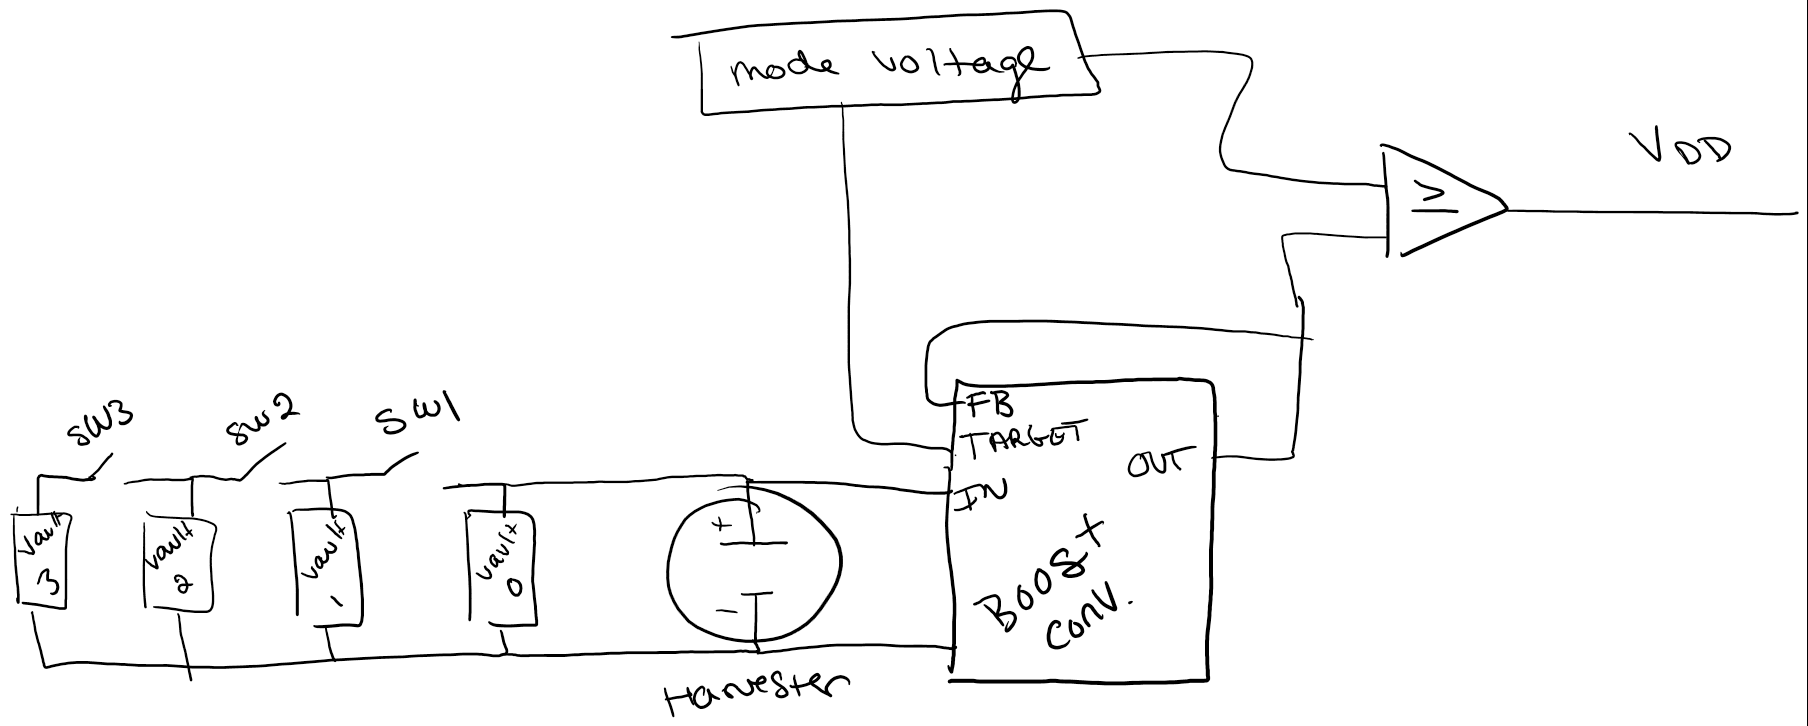
\includegraphics[width=0.95\textwidth,center]{capybara-all.png}
%\caption{Capybara power system overview}\label{label-a}
%\end{minipage}\hfill
%\begin{minipage}[b]{0.49\textwidth}
%  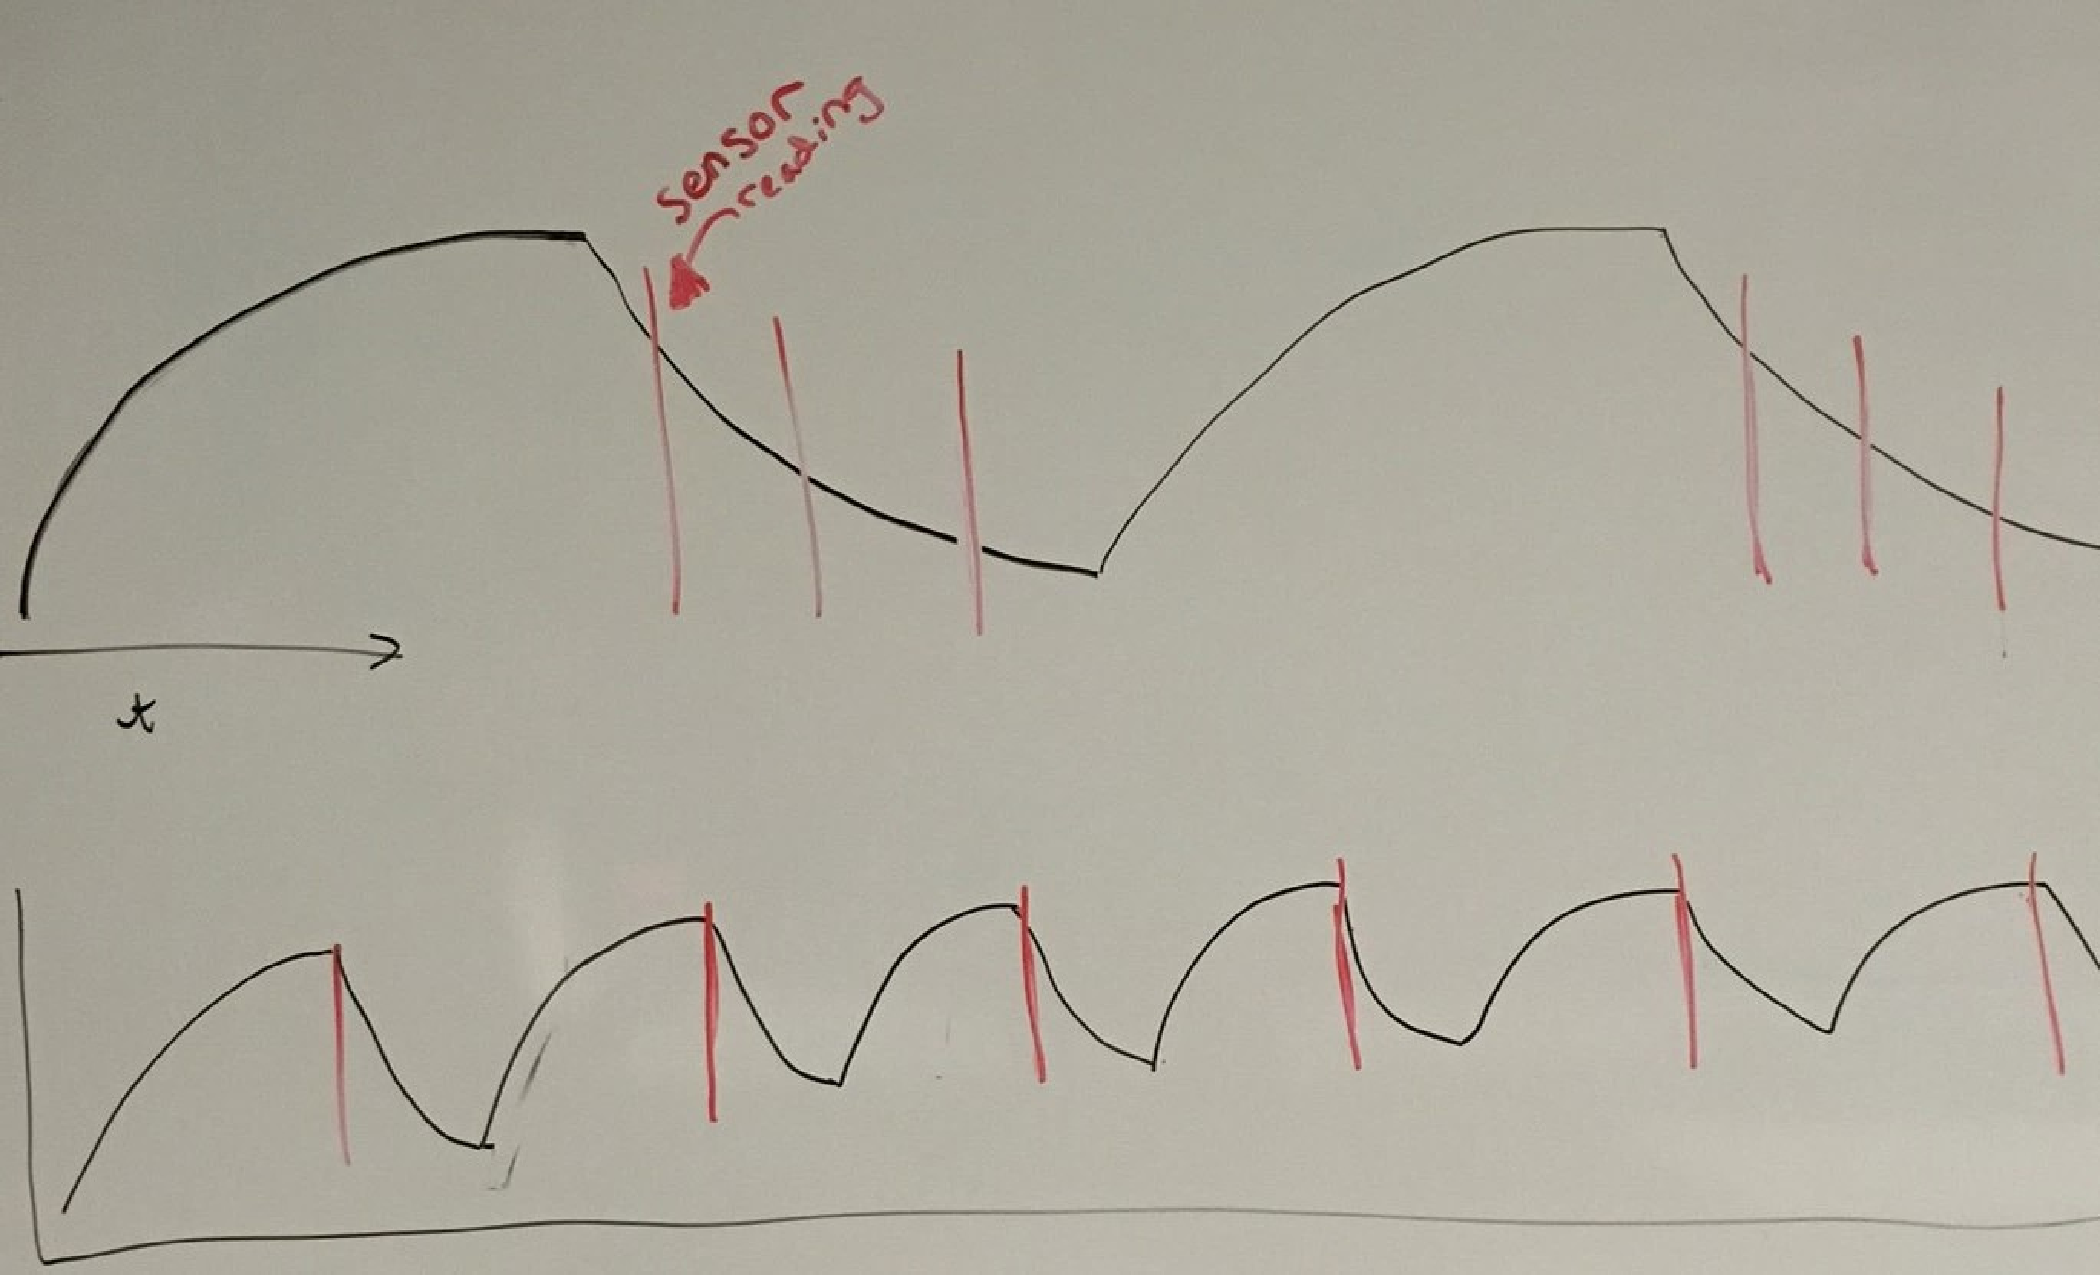
\includegraphics[width=0.95\textwidth,center]{power_modes.pdf}
%\caption{Effect of different power modes}\label{label-b}
%\end{minipage}
%\end{figure*}

More text after the picture to show how that looks...


\section{Related Work} -Emily
Operating system work\\
TU delft guys...\\
Energy Align\\


\section{Chain Discussion}
\chain, while providing a reasonable interface for programmers to work within,
has several inefficiencies that give poor performance on certain applications.
First, there is no notion of data sharing between tasks - all communication is
strictly done through channels. This is useful, as the programmer never needs
to reason about idempotence with respect to their data, but all data that needs
to be transferred between tasks needs to be housed in a channel. Since, under
the original constraints of \chain, channels cannot be written or read from by
tasks that do not own the channel - only tasks that own the channel can access
the data within. This means that large data structures, arrays for instance,
that need to be shared between several channels must be unnecessarily
duplicated in non-volatile memory - one copy of the data structure for each
channel that it needs to be accessed in. Granted, there is no enforcement of
channel ownership by the compiler, but the programmer risks idempotence
violations by straying outside the constraints of chain. We exploit this to
create an equivalent to the multicast-in and multicast-out channels described
in \chain, but using them requires much more reasoning on the part of the programmer.


Additionally, since dynamic memory allocation is arguably too expensive to run
on intermittently powered systems, memory is allocated at compile time.
Unfortunately, since there isn't a compiler specifically for \chain, arrays
are statically sized based on \texttt{\#define} parameters. This can be
create tricky memory corruption errors for the programmer when out-of-bounds
array accesses occur because, for instance, a self-channel has more dirty
fields than \texttt{MAX\_NUM\_DIRTY\_FIELDS}.


Future work for \chain needs to include some sort of memory allocation based on
the set of channels allocated in the program, but this is work for a compiler
and beyond the scope of this work. For our purposes of threaded applications,
however, \chain is a sufficient launching pad, despite its misgivings since it
does not require specialized hardware or energy subsystems to work effectively,
and since it solves the issue of idempotent data accesses in a way that is
abstracted from the programmer.


\section{What we did} % TODO change title
Scheduler\\
Mutexes - Emily\\
User programming model for threads - Neil\\
Round Robin (alternatives, on reboot)\\
SIMD vs MIMD\\
SIMD w/ channels (you don't get your own registers...etc -
    just channels, since intermittent)\\

\subsection{Interrupts}
\subsubsection{Motivation}
Ideally, multithreading would extend to a programming model that can utilize
interrupts in a producer/consumer fashion (i.e. a thread is waiting on data
from an external source, the external source fires an interrupt, the thread
samples the external source and stores the received data in a buffer, and
the thread returns to its original task). However, the inherent
non-deterministic
nature of interrupts from, say, an ADC, creates additional complexity for the
programmer when reasoning about shared memory, especially with respect to
idempotence.\\
    Specific to the MSP430 architecture (but common in other systems), there is
also the issue of stack integrity. On the MSP430, when an interrupt fires,
the program counter and status register are pushed onto the stack for
the handler to be able to return back to the state of the machine when the
interrupt fired. In our case, however, where power failure is the common
case, an application could experience failure while inside an interrupt
handler. This raises two issues. First, upon reboot from a power failure,
the stack will be cleared (since the stack is stored in volatile memory) and
execution will return to the handler, if we assume that the interrupt handler
is a \chain task. Upon leaving the interrupt, via the MSP430 RETI instruction),
the program's behavior will be undefined. Second, if the programmer does not
use a \chain task for the interrupt handler, it is possible that the interrupt
could fire when the system has a low amount of energy remaining, thus
rendering the system unable to finish executing the interrupt handler,
leading to a host of potential problems.

\subsubsection{Interface}
We provide the functions and macros in figure 3 as an interface to
the programmer. The standard workflow is as follows: the programmer
designates the task that should be run on an interrupt firing
with \texttt{INTERRUPT\_TASK(val, func)} where \texttt{val} is the task
index and \texttt{func} is the function that will be called upon an
interrupt firing - \texttt{val} and \texttt{func} follow the same
interface as \chain tasks. Since we assume that the handler is not
reentrant, the programmer replaces calls to \texttt{\_\_enable\_interrupt()}
with our function \texttt{enable\_interrupts()}.
The programmer's code remains unmodified, with the exception of a call to
\texttt{int\_setup\_complete()} when the \chain program has finished whatever
register initialization is necessary to setup the interrupts for the
application.\\

\begin{figure*}
\begin{minipage}[b]{0.49\textwidth}
\begin{lstlisting}
    /** Enable interrupts if int_setup_complete() has been called
      * and execution is not inside an interrupt handler */
    void enable_interrupts();

    /** To be called when setup for the interrupt handler is complete,
      * also enables interrupts */
    void int_setup_complete();

    /** Return from the interrupt handler */
    void return_from_interrupt();

    /** Designate a task to run when an interrupt fires */
    INTERRUPT_TASK(val, func)
\end{lstlisting}
\caption{Interrupt Handling Interface}\label{label-a}
\end{minipage}\hfill
\end{figure*}

\subsubsection{Design}
Working within the constraints of \chain and our multi-programming extensions,
we work to provide a layer of abstraction to the programmer through the standard
layer of tasks and channels. Notably, this includes interrupt handlers being
tasks, rather than standard functions. The alternative has been explored
by keeping specific capacitors for interrupt handlers\cite{Aware}, but this
approach fails if interrupt handlers take longer than the capacitor has
energy for. This bug handlers not completing due to power failure is
unintuitive for programmers coming from consistently powered devices and
makes certain devices unusable under intermittent power.\\
With interrupt handlers as tasks, if a power failure occurs during a
handler, execution will resume at the handler. This isn't ideal, the
standard paradigm that interrupt handlers are generally short and fast
so that interrupts won't be missed (for instance, a timer interrupt
being missed because processing the interrupt took longer than the
timer period), but we argue that it is more unreasonable to say
that interrupt handlers that take too long will not complete than
to violate the standard paradigm, since the former arbitrarily restricts
the application domain.


For the sake of simplicity, we assume that interrupt handlers are not
reentrant. Since reentrant handlers can be used in a non-reentrant fashion
without consequences, this assumption does not restrict the application domain.
Moreover, the benefit to reentrant handlers, the application will not miss an
interrupt firing because processing the previous one took too long, is
secondary on intermittent architectures - there is likely a higher chance that
a power failure will occur than an interrupt handler causing an interrupt to be
missed, unless interrupts are firing on an extremely fine granularity.


When an interrupt handler has completed, the programmer calls
\texttt{return\_from\_interrupt()}, which returns execution to the start
of the task that was running when the interrupt occurred. This contradicts
expected behavior - on continuously powered systems, execution generally
returns to the instruction after the instruction that the system received an
interrupt while processing. The continuous system model is intuitive, but
breaks under \chain's intermittence. Task idempotence in \chain only works
when execution returns to the top of a
task upon power failure. Program state (registers and stack memory) are stored
in volatile memory, if an interrupt handler returned to the middle of a task,
it would be impossible to reason about program correctness, since none of the
program state had been stored. The programmer could store program state on the
stack at the start of interrupt handlers, but this would be lost on power
failure. She could also store this program state in non-volatile memory -
trivial for the register set, but difficult and potentially extremely costly to
store the stack, as execution could be several functions deep. Even determining
how much stack to save could be prohibitively costly. Another alternative would
be to store program state in non-volatile, but this has been shown to be
prohibitively costly in most applications \cite{Aware}.


\section{Implementation}
We only had to break \chain a little. We promise!
Scheduler Data structures and idempotence (what we broke and why) -NEIL\\
Mutexes (Simple, meant for pseudo channels) - Emily\\
Interrupts (mucked with IE flags) - Neil\\
% Interrupt prologue
% Interrupt setup


\section{Results} - Emily
No really, there will be things here!
Applications/measurements\\
Blinker (x2)\\
RSA+cukoo\\
No verification\\
Memory overhead (read off compilation)\\
Performance (\# reboots)\\


\section{Future Work} -Amanda
Duplicating channels (a little renaming or sharing arrays with mutexes)\\
Optimizations to reduce overhead\\


\section{Conclusion}
Multithreading in intermittence {\em is} a good idea!


\balance
\bibliographystyle{abbrv}
\bibliography{sigproc}  % sigproc.bib is the name of the Bibliography
\end{document}
